\documentclass{standalone}

\begin{document}


\documentclass{standalone}

\begin{document}

\chapter[Deep Learning]{Deep Learning - Neural Network algorithms}\label{chapter2:neural}

Description of the modern deep neural networks.
Computational problems and potential applications

\end{document}
 % Neural Network introduction

\documentclass{standalone}

\begin{document}

\section[Neural Network models]{Neural Network models}\label{nn}

Neural Networks are mathematical models commonly used in data analysis.
They are becoming a standard tool in Machine Learning and Deep Learning research and many complex problems can be easily solved by these models.
From a theoretical point-of-view we can define a Neural Network as a series of non-linear multi-parametric functions.
The model parameters are tuned during a so called \emph{training section} in which we feed our model with a set of data with human supervision, i.e we have prior knowledge about the right and desired output of the model.
After the training section we can verify the efficiency of our training using a new set of data, called \emph{test set}, which is never seen by the model.
If we have prior knowledge about the output of our test set we can compute the accuracy (or more generally the score) of our model; in the other case we will simply have an extrapolation of our data.

A wide range of documentations and implementations have been written on this topic and it is more and more hard to move around the different sources.
Leader on this topic are became the multiple open-source Python libraries available on-line as \emph{Tensorflow}~\cite{tensorflow2015-whitepaper}, \emph{Pytorch}~\cite{paszke2017automatic} and \emph{Caffè}~\cite{Jia:2014:Caffe}.
Their portability and efficiency are closely related on the simplicity of the Python language and on the simplicity in writing complex models in a minimum number of code lines.
Only a small part of the research community uses more deeper implementation in C++ or other low-level programming languages.
About them it should be mentioned the \emph{darknet project} of Redmon J. et al. which created a sort of standard in object detection applications using a pure Ansi-C library.

In this section we firstly retrace the mathematical background of these models.
To each theoretical explanation we discuss the numerical problems associated and we provide an efficient custom implementation of each algorithm.
The numerical aspects will be traced following two  developed custom libraries: NumPyNet library~\cite{NumPyNet} and Byron library~\cite{Byron}.

NumPyNet was born as educational framework for the study of Neural Network models.
It is written trying to balance code readability and computational performances and it is enriched with a large documentation to better understand the functionality of each script.
The library is written in pure Python and the only external library used is Numpy~\cite{Numpy} (a based package for the scientific research).

Despite all common libraries are correlated by a wide documentation is often difficult for novel users to move around the many hyper-links and papers cite in it.
NumPyNet tries to overcome this problem with a minimal mathematical documentation associated to each script and a wide range of comments inside the code.

An other \quotes{problem} to take in count is related to performances.
Libraries like \emph{Tensorflow} as certainly efficient by a computational point-of-view and the numerous wrappers (like \emph{Keras} library) guarantees an extremely simple user interface.
On the other hand the deeper functionality of the code and the implementation strategies used are unavoidably hidden behind tons of code lines.
In this way the user can performs complex computational tasks using the library as black-box package.
NumPyNet wants to overcome this problem using simple Python codes with extremely readability also for novel users to better understand the symmetry between mathematical formulas and code.

The simplicity of this library we will allow to give a first numerical analysis of the model functions and, moreover, to show the results of each function to a simple image to better understand the effects of their applications on real data\footnote{
  Aware of the author no other example implementations have been done.
  This makes the NumPyNet library a useful tool for neural network study and a virtual laboratory for new neural network functions.
}.
Each NumPyNet function was tested against the \emph{Tensorflow} implementation of the same methods with an automatic testing routine through \emph{PyTest}~\cite{Okken:2017:PTP:3176124}.
The full code is open-source on the Github page of the project.
Its installation is guaranteed by a continuous integration framework of the code through \emph{Travis CI} for Unix environments and \emph{Appevyor CI} for Windows users.
The library supports Python version $\ge2.6$\footnote{
  The library provides also an \textsf{Image} object to load and process images.
  The object is based on OpenCV API~\cite{OpenCV}.
  OpenCV does not yet support Python version 2.7 and 3.3 so the whole NumPyNet package does not work on these two version of Python.
  You can just exclude the \textsf{Image} scripts from the package or use a novel wrap based on different library (e.g \textsf{Pillow}).
}.

As term of comparison we will discuss the more sophisticated implementations into the Byron library.
Byron (Build YouR Own Neural network) library is written in pure C++ with the support of the modern standard 17.
We deeply use the c++17 functionality to reach the better performances and flexibility of our code.
What makes Byron an efficient alternative to the competition is the complete multi-threading environment in which it works.
Despite the most common Neural Network libraries are optimized for GPU environments, there are only few code implementations which exploit the fully functionality of a multiple CPUs architecture.
This gap discourage multiple research groups on the use of such computational intensive models in their applications.
Byron works in a fully parallel section in which is single computational function is performed using the full set of available cores.
To further reduce the time of thread spawn and so optimize as much as possible the code performances, the library works using a single parallel section which is opened at the beginning of the computation and closed at the end\footnote{
  For real-time applications also the time required for the thread spawn must be taken into account.
}.

The Byron library is release under MIT license and public available on the Github page of the project.
The project also includes a list of common examples like object detection, super resolution, segmentation, ecc. (see the next sections for further details about this models).
The library is also completely wrapped using \emph{Cython} to enlarge the range of users also to the Python ones.
The complete guide to its installation is provided; it can be done using \emph{CMake}, \emph{Make} or \emph{Docker} and the Python version is available with a simple \emph{setup}.
The testing of each function is performed using \emph{Pytest} automatic framework against the NumPyNet implementation (faster and lighter to import than \emph{Tensorflow}).

We will use Byron library as term of comparison with the other common library used in Neural Network models and for each function we test its computational efficiency and scalability on multiple cores.
Two machines will be used in the computational testing: a common laptop (8~GB RAM memory and 1 CPU i7-6500U, with 2 cores) and a classical bioinformatics server (128~GB RAM memory and 2 CPU E5-2620, with 8 cores each).

Starting from the next section we introduce the fundamental Neural Network model, the so-called \emph{Simple Perceptron}.
From the simplest model we will add complexity layers to overcome the relative problems (mathematical and numerical), introducing the main functionality of the modern Neural Network architectures.

\end{document}

\documentclass{standalone}

\begin{document}

\subsection[Simple Perceptron]{Simple Perceptron}\label{NN:perceptron}

The fundamental unit of each Neural Network model is the \emph{simple Perceptron} (or single neuron).
The \emph{Perceptron} is the simpler mathematical model of biological neuron and it is based on the Rosenblatt~\cite{Rosenblatt58theperceptron} model which identifies a neuron as a computational unit with input, synaptic weights and an activation threshold (or function).
Following the biological model of Hodgkin and Huxley~\cite{HHmodel} (H-H model), we have an action potential, i.e the output of the neuron, given by

$$
y = \sigma\left(\sum_{i=1}^{N}w_i x_i + w_0 \right)
$$
\\
where $\sigma$ is the activation function, $w_i$ are the synaptic weights and $x_i$ the inputs.
The $w_0$ coefficient identifies the bias of the linear combination and it is left as parameter to be tune by the optimization algorithm (learning phase).

The connection weights $w_i$ are tuned during the training section by the chosen updating rule.
The standard updating rule is simply given by

$$
w_i(\tau + 1) = w_i(\tau) + \gamma(t - y)x
$$
\\
where $\gamma$ is the gain or step size ($\gamma \in [0, 1]$) and $t$ is the desired output.
In other words we have to compute firstly the difference between the current output and the desired one, i.e the error or cost function or loss function\footnote{
  There are multiple loss functions in the Neural Network world.
  We will further discuss their use and their effective on a learning model in the next section.
}, and weight this error by the gain factor and the corresponding input.
Repeating the error computation and the updating rule we can bring the weights to convergence.
From a geometrical point-of-view this process is equivalent to an hyper-plane placement defined by $w_0 + < w, x >$ which splits an $n-$dimensional space into two half-spaces, i.e two desired classes.

The mathematical formulation already highlights the numerous limits of this model.
The output function is a simple linear combination of the input with a vector of weights, and so only linearly separable problems can be learned\footnote{
  A simple mathematical proof of it can be found \href{http://www.cs.columbia.edu/~mcollins/courses/6998-2012/notes/perc.converge.pdf}{here}.
} by the \emph{Perceptron}\footnote{
  A classical example of learning problems is given by the XOR logic function.
  Since the XOR output is not linearly separable the Perceptron could not converge.
}.
Moreover we can manage only two classes since an hyper-plane divide the space in only two half-spaces.

A key role is assumed by the activation function.
The classical activation function used in the discrete Perceptron model is the \emph{unit step function} (or \emph{Heaviside step function}).
If we chose a continuous and so differentiable activation function we can treat the problem using a continuous cost function.
In this case we define it as

$$
E(\mathbf{w}) = \frac{1}{2}\sum_{i=1}^{N}\left( t_i - y_i \right)^2
$$
\\
where in this case both $t_i$ and $y_i$ are continuous variables, i.e floating point numbers.
Now, the updating rule can be given by the gradient of the cost function applied to the original weights as

$$
\mathbf{w} = \mathbf{w} + \Delta\mathbf{w}
$$
\\
where $\Delta\mathbf{w}$ is given by

$$
\Delta\mathbf{w_i} = -\gamma\frac{\partial E}{\partial w_i} = -\gamma\sum_{i=1}^{N} \left( t_i - y_i \right)\left(-x_i \right)
$$
\\
which looks identical to previous updating rule but in this case we are managing real numbers and not simple class labels.
In this way we compute the weight updates according to the full set of training samples and not for each sample (this approach leads to the so-called \emph{batch}-update, i.e small subsets of data).

To implement this kind of model into a pure \textsf{Python} application we do not need extra libraries, but we can just use the native keywords of the language.
A possible implementation of this model was developed and release in an on-line \href{https://gist.github.com/Nico-Curti/358b7a2ffed1abbb57ee87a5338ca073}{gist}.
In this simple snippet we examine the functionality of the Simple Perceptron model across different logical functions and we proved its fast convergence on linear separable datasets\footnote{
  We proof the non-linear separable convergence introducing an extra stop criteria during the weights tuning given by a maximum number of step.
}.
An equivalent \textsf{C++} implementation of the model is also released and it can be found in this other \href{https://gist.github.com/Nico-Curti/856c3baf523bc5d01b1e7dfe2515c0e2}{gist}.

The model is too naive for computational efficiency discussions.
Thus we just observe how a learning algorithm could be easily implemented using basic programming language keywords either in \textsf{Python} and \textsf{C++}.

\end{document}

\documentclass{standalone}

\begin{document}

\section[Fully Connected Neural Network]{Fully Connected Neural Network}\label{NN:connected}

To overcome problems arising from the Simple Perceptron model we can join together multiple Perceptron units into a more complex network of interaction in which the output of a neuron feed-forward the input of the next one.
This is the Multi-layers Perceptron (MLP) configuration and if the graph is fully connected, i.e each neuron is connected to all the others, we talk about \emph{fully connected neural networks} (or \emph{dense} neural network, DNN).

Given the Perceptron formulas, the extrapolation to the MLP architecture is straight-forward and given by

$$
y = \sigma\left(X \cdot W + W_0 \right)
$$
\\
where we simply pass from the vector formulation to the matrix one.
The updating rule consequentially becomes

$$
\delta W = \delta W + X^T \cdot \left( \frac{\partial f(y)}{\partial y} \cdot \delta^l \right)  \quad\quad \delta W_0 = \sum_{i=0}^{m}\frac{\partial f(y)}{\partial y_i} \cdot \delta_i^l
$$
\\
where also in this case we simply pass to the matrix formalism and we convert the discrete format to a continuous one, i.e with continuous values we convert the error to a partial derivative.
In the above equation $\delta^l$ represents the error pass from the next layer in the network structure\footnote{
  In the Back-Propagation Algorithm the error is passed by each layer to the previous one, starting from the output error computed according to chosen loss function.
}.

From the re-iteration of such structures we can join together multiple fully connected layers and so obtain multiple neuron layers jointly together with different levels of complexity and units (an input layer followed by multiple \emph{hidden} layers).

The fully connected Neural Networks overcome the told above \emph{Perceptron} problems using a combination of linear functions (single \emph{Perceptron} units) and they gain more useful properties:

\begin{itemize}

\item If the activation functions of \emph{all} the hidden units in the Neural Network are linear, then the network architecture is equivalent to a network without hidden units.

\item If the number of hidden units is smaller than either the number of input units either the number of output ones, then the network can generate transformations from inputs to outputs as much general as possible since the information is lost in the dimensionality reduction performed by the hidden units.

\item We can find multiple weight configurations, i.e $W$ matrices, which give us the same mapping function from inputs to outputs.

\end{itemize}


\end{document}

\documentclass{standalone}

\begin{document}


\subsubsection[Matrix Product]{Matrix Product}\label{NN:gemm}

Despite the mathematical formulation of the model we have to take into account also an efficient implementation.
From a numerical point-of-view we can notice that all the computation required by this kind of Networks (or layer if we consider it into an hybrid Neural Network architecture as we will see in the next sections) can be summarized into the matrix product evaluation.
The matrix product is a well-known numerical problem and its algorithmic complexity can be hardly reduced under $O(N^3)$\footnote{
  The complexity is often given in the assumption of only square matrices $(N\times N)$ involved in the computation.
  For no-square matrix the algorithm complexity is given by the product of the three possible different matrix dimensions involved ($(N\times K) = (N\times M)(M\times K)$ brings to $O(NMK)$ complexity).
  More sophisticated implementation of the algorithm are able to reduce the algorithm complexity (e.g Strassen algorithm) but neither implementation is able to overcome the $O(N^{2.7})$ complexity up-to-now.
}.
A crucial role on this kind of algorithms is played by the cache accesses.
The CPU cache is the hardware cache used by the CPU to store small portion of data in order to reduce the average cost (in time or energy consumption) to data access from the main memory.
Cache optimization is one of the most difficult parts to perform writing an algorithm, but it leads to highest performance gains.

In the matrix product we have to multiply each row of a matrix $A$ by each column of a second matrix $B$.
We work in the assumption that each matrix is stored into an array of 1D or 2D without nested structures.
In this case we can access to a contiguous memory portion of the first matrix since each row is given by a series of sequential index locations (the row elements are given by $x[0], x[1], \dots, x[N]$).
This configuration allows the cache optimization in the access to the first matrix, since we can store in a small portion of cache memory a series of row elements and use them in a vectorization environment.

From the second matrix we have to extract the elements from each column.
This means that the elements are given by a discontinuous portion of memories (the column elements are given by $x[0], x[M], x[2M], \dots, x[N(M-1)]$).
In this case we can not insert a full column into the cache memory and in consequence we have a \emph{cache-miss} at each iteration\footnote{
  The \emph{cache-miss} happens when a required data can not be found into the cache and so its search has to be done in the main memory (RAM).
}.

The simple matrix product as given by row-column multiplication is already affected by an intrinsic numerical problem which can drastically affect its performances.
The simplest workaround of this issue is to perform a transposition of the second matrix to obtain a row-row matrix product\footnote{
  In the discussion we have silently ignored the problems of matrix storage and the cache optimization for the resulting matrix accesses but in the above discussion we want to focus only on the main problems raising from the matrix product.
}.
In this way both matrices can be accessed in a sequential order.
The total complexity of the computation increase to $O(N^2)$ (for the matrix transposition, in the better case) $+ O(N^3)$ (for matrix product) but the numerical performances increase due to the cache-miss minimization\footnote{
  The cache memory is a very tight portion of memory and it is impossible to completely remove cache-misses.
}.

Following back to our Neural Network implementation we can obtain the output values using the above technique.
Moreover, we can assume from the beginning that the transposition of weight matrix and so remove the $O(N^2)$ calculus from the matrix product.
This simple (but carefully studied) optimization allows to obtain better results in the feed-forward evaluation, but it paybacks a revision of the standard mathematical formulation and a carefully implementation of the code.

\begin{figure}[htbp]
\includegraphics[width=0.45\textwidth]{GEMM_schema.png}
\quad
\centering
\def\svgwidth{0.45\textwidth}
\documentclass{standalone}

\begin{document}


\subsubsection[Matrix Product]{Matrix Product}\label{NN:gemm}

Despite the mathematical formulation of the model we have to take into account also an efficient implementation.
From a numerical point-of-view we can notice that all the computation required by this kind of Networks (or layer if we consider it into an hybrid Neural Network architecture as we will see in the next sections) can be summarized into the matrix product evaluation.
The matrix product is a well-known numerical problem and its algorithmic complexity can be hardly reduced under $O(N^3)$\footnote{
  The complexity is often given in the assumption of only square matrices $(N\times N)$ involved in the computation.
  For no-square matrix the algorithm complexity is given by the product of the three possible different matrix dimensions involved ($(N\times K) = (N\times M)(M\times K)$ brings to $O(NMK)$ complexity).
  More sophisticated implementation of the algorithm are able to reduce the algorithm complexity (e.g Strassen algorithm) but neither implementation is able to overcome the $O(N^{2.7})$ complexity up-to-now.
}.
A crucial role on this kind of algorithms is played by the cache accesses.
The CPU cache is the hardware cache used by the CPU to store small portion of data in order to reduce the average cost (in time or energy consumption) to data access from the main memory.
Cache optimization is one of the most difficult parts to perform writing an algorithm, but it leads to highest performance gains.

In the matrix product we have to multiply each row of a matrix $A$ by each column of a second matrix $B$.
We work in the assumption that each matrix is stored into an array of 1D or 2D without nested structures.
In this case we can access to a contiguous memory portion of the first matrix since each row is given by a series of sequential index locations (the row elements are given by $x[0], x[1], \dots, x[N]$).
This configuration allows the cache optimization in the access to the first matrix, since we can store in a small portion of cache memory a series of row elements and use them in a vectorization environment.

From the second matrix we have to extract the elements from each column.
This means that the elements are given by a discontinuous portion of memories (the column elements are given by $x[0], x[M], x[2M], \dots, x[N(M-1)]$).
In this case we can not insert a full column into the cache memory and in consequence we have a \emph{cache-miss} at each iteration\footnote{
  The \emph{cache-miss} happens when a required data can not be found into the cache and so its search has to be done in the main memory (RAM).
}.

The simple matrix product as given by row-column multiplication is already affected by an intrinsic numerical problem which can drastically affect its performances.
The simplest workaround of this issue is to perform a transposition of the second matrix to obtain a row-row matrix product\footnote{
  In the discussion we have silently ignored the problems of matrix storage and the cache optimization for the resulting matrix accesses but in the above discussion we want to focus only on the main problems raising from the matrix product.
}.
In this way both matrices can be accessed in a sequential order.
The total complexity of the computation increase to $O(N^2)$ (for the matrix transposition, in the better case) $+ O(N^3)$ (for matrix product) but the numerical performances increase due to the cache-miss minimization\footnote{
  The cache memory is a very tight portion of memory and it is impossible to completely remove cache-misses.
}.

Following back to our Neural Network implementation we can obtain the output values using the above technique.
Moreover, we can assume from the beginning that the transposition of weight matrix and so remove the $O(N^2)$ calculus from the matrix product.
This simple (but carefully studied) optimization allows to obtain better results in the feed-forward evaluation, but it paybacks a revision of the standard mathematical formulation and a carefully implementation of the code.

\begin{figure}[htbp]
\includegraphics[width=0.45\textwidth]{GEMM_schema.png}
\quad
\centering
\def\svgwidth{0.45\textwidth}
\documentclass{standalone}

\begin{document}


\subsubsection[Matrix Product]{Matrix Product}\label{NN:gemm}

Despite the mathematical formulation of the model we have to take into account also an efficient implementation.
From a numerical point-of-view we can notice that all the computation required by this kind of Networks (or layer if we consider it into an hybrid Neural Network architecture as we will see in the next sections) can be summarized into the matrix product evaluation.
The matrix product is a well-known numerical problem and its algorithmic complexity can be hardly reduced under $O(N^3)$\footnote{
  The complexity is often given in the assumption of only square matrices $(N\times N)$ involved in the computation.
  For no-square matrix the algorithm complexity is given by the product of the three possible different matrix dimensions involved ($(N\times K) = (N\times M)(M\times K)$ brings to $O(NMK)$ complexity).
  More sophisticated implementation of the algorithm are able to reduce the algorithm complexity (e.g Strassen algorithm) but neither implementation is able to overcome the $O(N^{2.7})$ complexity up-to-now.
}.
A crucial role on this kind of algorithms is played by the cache accesses.
The CPU cache is the hardware cache used by the CPU to store small portion of data in order to reduce the average cost (in time or energy consumption) to data access from the main memory.
Cache optimization is one of the most difficult parts to perform writing an algorithm, but it leads to highest performance gains.

In the matrix product we have to multiply each row of a matrix $A$ by each column of a second matrix $B$.
We work in the assumption that each matrix is stored into an array of 1D or 2D without nested structures.
In this case we can access to a contiguous memory portion of the first matrix since each row is given by a series of sequential index locations (the row elements are given by $x[0], x[1], \dots, x[N]$).
This configuration allows the cache optimization in the access to the first matrix, since we can store in a small portion of cache memory a series of row elements and use them in a vectorization environment.

From the second matrix we have to extract the elements from each column.
This means that the elements are given by a discontinuous portion of memories (the column elements are given by $x[0], x[M], x[2M], \dots, x[N(M-1)]$).
In this case we can not insert a full column into the cache memory and in consequence we have a \emph{cache-miss} at each iteration\footnote{
  The \emph{cache-miss} happens when a required data can not be found into the cache and so its search has to be done in the main memory (RAM).
}.

The simple matrix product as given by row-column multiplication is already affected by an intrinsic numerical problem which can drastically affect its performances.
The simplest workaround of this issue is to perform a transposition of the second matrix to obtain a row-row matrix product\footnote{
  In the discussion we have silently ignored the problems of matrix storage and the cache optimization for the resulting matrix accesses but in the above discussion we want to focus only on the main problems raising from the matrix product.
}.
In this way both matrices can be accessed in a sequential order.
The total complexity of the computation increase to $O(N^2)$ (for the matrix transposition, in the better case) $+ O(N^3)$ (for matrix product) but the numerical performances increase due to the cache-miss minimization\footnote{
  The cache memory is a very tight portion of memory and it is impossible to completely remove cache-misses.
}.

Following back to our Neural Network implementation we can obtain the output values using the above technique.
Moreover, we can assume from the beginning that the transposition of weight matrix and so remove the $O(N^2)$ calculus from the matrix product.
This simple (but carefully studied) optimization allows to obtain better results in the feed-forward evaluation, but it paybacks a revision of the standard mathematical formulation and a carefully implementation of the code.

\begin{figure}[htbp]
\includegraphics[width=0.45\textwidth]{GEMM_schema.png}
\quad
\centering
\def\svgwidth{0.45\textwidth}
\input{./img/gemm.pdf_tex}
\caption{GEMM algorithms time performances.
\textsf{GEMM NN}: matrix multiplication considering both the matrices in \quotes{normal} format, i.e $A\cdot B$.
\textsf{GEMM NT}: matrix multiplication considering the first matrix in \quotes{normal} format and the second one transposed, i.e $A\cdot B^T$.
We perform 100 tests of 1K runs each of both the \textsf{GEMM} algorithms using the \textsf{einsum} function of \textsf{Numpy} library.
The values are rescaled according to the mean time of the \textsf{GEMM NN} algorithm.
}
\label{fig:gemm}
\end{figure}

In the proposed numerical implementations of this model we implement both the matrix product cases to compare the performance results.
We tested the two implementations inside \textsf{Python} using the \textsf{einsum} function provided by the \textsf{Numpy} package.
In particular, we evaluated the time-performances over 1000 applications of the two \textsf{GEMM} functions (\textsf{GEMM NN}, i.e considering both matrices with \quotes{normal} shapes; \textsf{GEMM NT}, i.e considering the first matrix as \quotes{normal} and the second transposed) considering matrices of shapes ($100\times100$).
We performed $500$ run and we saved the minimum time obtained over $10$ realizations.
In Fig.~\ref{fig:gemm} we show the results rescaled by the mean time (over the 500 realizations) of the \textsf{GEMM NN} algorithm (reference).
As can be seen in Fig.~\ref{fig:gemm} the speedup of the \textsf{GEMM NT} matrix is evident and it is always faster than \textsf{GEMM NN} algorithm with a maximum of $3.2$x in the speedup.

In the \textsf{Byron} library we provide a parallelized version of this algorithm with also an \textsf{avx} support.
In this way we could manually manage the register memory of the two matrices and obtain a faster \textsf{GEMM} algorithm (especially for dimensions proportional to powers of 2 which are very common in neural network models).

\end{document}

\caption{GEMM algorithms time performances.
\textsf{GEMM NN}: matrix multiplication considering both the matrices in \quotes{normal} format, i.e $A\cdot B$.
\textsf{GEMM NT}: matrix multiplication considering the first matrix in \quotes{normal} format and the second one transposed, i.e $A\cdot B^T$.
We perform 100 tests of 1K runs each of both the \textsf{GEMM} algorithms using the \textsf{einsum} function of \textsf{Numpy} library.
The values are rescaled according to the mean time of the \textsf{GEMM NN} algorithm.
}
\label{fig:gemm}
\end{figure}

In the proposed numerical implementations of this model we implement both the matrix product cases to compare the performance results.
We tested the two implementations inside \textsf{Python} using the \textsf{einsum} function provided by the \textsf{Numpy} package.
In particular, we evaluated the time-performances over 1000 applications of the two \textsf{GEMM} functions (\textsf{GEMM NN}, i.e considering both matrices with \quotes{normal} shapes; \textsf{GEMM NT}, i.e considering the first matrix as \quotes{normal} and the second transposed) considering matrices of shapes ($100\times100$).
We performed $500$ run and we saved the minimum time obtained over $10$ realizations.
In Fig.~\ref{fig:gemm} we show the results rescaled by the mean time (over the 500 realizations) of the \textsf{GEMM NN} algorithm (reference).
As can be seen in Fig.~\ref{fig:gemm} the speedup of the \textsf{GEMM NT} matrix is evident and it is always faster than \textsf{GEMM NN} algorithm with a maximum of $3.2$x in the speedup.

In the \textsf{Byron} library we provide a parallelized version of this algorithm with also an \textsf{avx} support.
In this way we could manually manage the register memory of the two matrices and obtain a faster \textsf{GEMM} algorithm (especially for dimensions proportional to powers of 2 which are very common in neural network models).

\end{document}

\caption{GEMM algorithms time performances.
\textsf{GEMM NN}: matrix multiplication considering both the matrices in \quotes{normal} format, i.e $A\cdot B$.
\textsf{GEMM NT}: matrix multiplication considering the first matrix in \quotes{normal} format and the second one transposed, i.e $A\cdot B^T$.
We perform 100 tests of 1K runs each of both the \textsf{GEMM} algorithms using the \textsf{einsum} function of \textsf{Numpy} library.
The values are rescaled according to the mean time of the \textsf{GEMM NN} algorithm.
}
\label{fig:gemm}
\end{figure}

In the proposed numerical implementations of this model we implement both the matrix product cases to compare the performance results.
We tested the two implementations inside \textsf{Python} using the \textsf{einsum} function provided by the \textsf{Numpy} package.
In particular, we evaluated the time-performances over 1000 applications of the two \textsf{GEMM} functions (\textsf{GEMM NN}, i.e considering both matrices with \quotes{normal} shapes; \textsf{GEMM NT}, i.e considering the first matrix as \quotes{normal} and the second transposed) considering matrices of shapes ($100\times100$).
We performed $500$ run and we saved the minimum time obtained over $10$ realizations.
In Fig.~\ref{fig:gemm} we show the results rescaled by the mean time (over the 500 realizations) of the \textsf{GEMM NN} algorithm (reference).
As can be seen in Fig.~\ref{fig:gemm} the speedup of the \textsf{GEMM NT} matrix is evident and it is always faster than \textsf{GEMM NN} algorithm with a maximum of $3.2$x in the speedup.

In the \textsf{Byron} library we provide a parallelized version of this algorithm with also an \textsf{avx} support.
In this way we could manually manage the register memory of the two matrices and obtain a faster \textsf{GEMM} algorithm (especially for dimensions proportional to powers of 2 which are very common in neural network models).

\end{document}


\input{./tex/Chapter2/NeuralNetwork/Activations.tex}
\documentclass{standalone}

\begin{document}


\subsection[Relu]{Rectified Linear Unit}\label{relu}

The ReLU (Rectified Linear Unit) activation functions are the most used into the modern Neural Networks models.
Their diffusion is imputed to their numerical efficiency and to the benefits they bring~\cite{}:

\begin{itemize}

\item Information disentangling: the main purpose of a Neural Network model is to tune a discriminant function able to associate a set of input to a prior-known output classes.
A dense information representation is considered \emph{entangled} because small differences in input highly modifies the data representation inside the network.
On the other hand, a sparse representation tends to guarantee a conservation of the learning features.

\item Information representation: different inputs can lead different quantities of useful informations.
The possibility to have null values in output (ref Tab.~\ref{tab:activations}) allows a better representation of the representation dimension inside the network.

\item Sparsity: sparsity representation of data are exponentially efficient in comparison to dense ones, where the exponential power is given by the number of no-null features~\cite{}.

\item Vanish gradient reduction: if the activation output is positive we have a no-bound gradient value.
%add other considerations

\end{itemize}

\end{document}


\documentclass{standalone}

\begin{document}

\section[Dropout function]{Dropout function}\label{NN:dropout}

Many times along this work we have been talked about the \emph{over-fitting} problem.
The over-fitting problems arise when the complexity of our model becomes too high regard the amount of available data, i.e when the number of parameters of our model is comparable to the number of available data.
A classical example is given by the polynomial fitting problem.
Given an initial set of $N$ data points we can always find a polynomial curve of degree equal to $N-1$ which can perfectly fit our data.
In this case the model flexibility is minimum and new additional data points difficulty lies on the same curve.
In other words we tuned each model parameter according to the given data set but we completely lose the possibility of generalization.

In Neural Network models we have to manage a large quantities of parameters and it is quite easy to stumble on this problem.
A possible workaround is given by a Dropout function.
This function simply dropping out some neuron units into a neural network during the training phase.
Ignoring some neurons means that they will not be considered during a particular (single) forward/backward step.
So, given a set of neuron we have a probability $p$ to keep the neuron and $1-p$ to remove it.
In this way we can reduce the co-dependency of nearest neurons inside the network and so reduce the possibility of over-fitting.
An other common way is to regularize the neuron outputs with penalty loss function\footnote{
  Classical examples are given by the L1 (Laplacian) and L2 (Gaussian) penalties.
  Both these functions are implemented either in NumPyNet and Byron but for sake of brevity we will not discuss about them.
}.



\subsection[Numerical Implementation]{Numerical Implementation}\label{NN:drop_num}

The above description bring us to a straight forward implementation of the algorithm into the NumPyNet library.


\lstset{style=snippet}
\begin{lstlisting}[language=Python, caption=NumPyNet version of Dropout function, label=code:py_dropout]
import numpy as np

class Dropout_layer(object):

  def __init__(self, prob, **kwargs):

    self.probability = prob
    self.scale = 1. / (1. - prob)

    self.batch, self.w, self.h, self.c = (0, 0, 0, 0)

    self.output, self.delta = (None, None)

  def forward(self, inpt):

    self.batch, self.w, self.h, self.c = inpt.shape

    self.output = inpt.copy()

    self.rnd = np.random.uniform(low=0., high=1., size=self.output.shape) < self.probability
    self.output[self.rnd] = 0.
    self.rnd = ~self.rnd
    self.output[self.rnd] *= self.scale

  def backward(self, delta=None):

    if delta is not None:
      delta[self.rnd] *= self.scale
      self.rnd = ~self.rnd
      delta[self.rnd] = 0.

\end{lstlisting}

The above code numerically reproduce the theoretical formulation given.
After the initialization of the private object variables the forward function generate a set of random positions and apply them (if they are less than the given probability) to the output: these positions will be turned off and the others will be multiply by a scale probability factor to increase their importances.
The backward function simply invert the transformation on the back-propagated gradient \textsf{delta}.

Despite this straight forward implementation we have to carefully manage some crucial points into the C++ equivalent.
We are working on a complete parallel region so after the (sequential) initialization initialization of the layer object the forward/backward phases are evaluated by all the available threads in parallel.
This bring us to a standard problem in multi-threading programming: the generation of independent random numbers among threads.
Inside a parallel region all the variables declared are (by definition) shared among threads and so if we simply create a random number generator in it we have to face on the thread-concurrency.
As consequence the random number generated will not be independent but (most probably) repeated by each thread\footnote{
  The deterministic generation of random number is hard to reproduce into a parallel environments despite the seed initialization.
  The \quotes{probability} of repeat the same sequence is related to the affinity of each thread to the given process.
}.
The simple workaround implemented into Byron library is given by assigning a random number generator to each thread (with its own seed and indexed by the thread Id).
In this way we can ensure a totally independence of the random numbers generated during the forward phase (ref. \href{https://github.com/Nico-Curti/Byron/blob/master/src/dropout_layer.cpp}{on-line}).

\begin{figure}[htbp]
\centering
\def\svgwidth{0.7\textwidth}
\input{./img/dropout_layer.pdf_tex}
\caption{Dropout function applied on a testing image.
The 10\% of image pixels are turned off by the forward function.
The corresponding gradient is back-propagated only on the previously activated pixels.
}
\label{fig:dropout}
\end{figure}

As visualization example we can use a simple test image and apply our transformation (see Fig.\ref{fig:dropout}).
As expected our input image shows many pixel turned off according to the given probability.



\end{document}
 % talk about rng in parallel

\documentclass{standalone}

\begin{document}

% https://victorzhou.com/blog/intro-to-cnns-part-1/
% https://towardsdatascience.com/a-comprehensive-guide-to-convolutional-neural-networks-the-eli5-way-3bd2b1164a53
% https://ujjwalkarn.me/2016/08/11/intuitive-explanation-convnets/

\subsection[Convolution function]{Convolution function}\label{NN:convolutional}

A big revolution into the Neural Network research field has been given by the introduction of convolution functions.
Convolutional Neural Network (CNN) are particularly designed for image analyses.
Convolution is the mathematical integration of two functions in which the second one is translated by a given value:

\begin{equation}
(f * g)(t) = \int_{-\infty}^{+\infty} f(\tau)g(t - \tau)d\tau
\end{equation}

In signal processing, this operation is also called \emph{crossing correlation} ad it is equivalent to the \emph{autocorrelation} function computed at a given point.
In image processing the first function is represented by the image $I$ and the second one is a kernel $k$ (or filter), which shifts along the image.
In this case we have a 2D discrete version of the formula given by:

\begin{equation}
\begin{aligned}
C = k * I
\\
C[i, j] = \sum_{u=-N}^{N} \sum_{v=-M}^{M} k[u, v] \cdot I[i - u, j - v]
\end{aligned}
\end{equation}
\\
where $C[i, j]$ is the pixel value of the resulting image and $N$, $M$ are the kernel dimensions.

The use of CNN in modern image analyses can be traced back to multiple causes.
First of all the image dimensions are increasingly bigger and thus the number of variables/features, i.e pixels, is often too big to manage with standard DNN\footnote{
  If we consider a simple image $224\times224$ with $3$ color channels we obtain a set of \numprint{150528} features.
  A classical DNN layer with this input size should have $1024$ nodes for a total of more than $150$ million weights to tune.
}.
Moreover, if we consider detection problems, i.e the problem of detecting a set of features (or an object) into a larger pattern, we want a system ables to recognize the object regardless of where it appears into the picture.
In other words, we want that our model would be independent by simple translations.

Both the above problems can be overcame by CNN models using a small kernel, i.e weight mask, which maps the full input.
A CNN is able to successfully capture the spatial and temporal dependencies in a signal through the application of relevant filters.

The main parameters of this function are given by the input dimensions and the filter/kernel dimensions, i.e the number of weights which we have to tune during the training.
This is the basic idea behind the convolution function, but in many cases (especially in modern deep learning Neural Networks) we can sophisticate it, playing with the possible movements of the filter mask.
In particular, aside the kernel mask-size, we can force the filter to jump along the image, i.e a discontinuous movement of the filter excluding some pixels.
This parameter, called \textsf{stride}, defines the number of pixels to jump and it is often used to further reduce the output dimensions.

Given this theoretical background we can implement the convolution function in many different ways, using different mathematical approaches: a study about the computational efficiency will tell us which is the best approach to choose.
The first (naive) approach is to use a brute force technique and implement the direct evaluation of the convolution function as described in the above equation.
This version is certainly the easier to implement, but its computational performances are so worst that, for sake of brevity, we excluded it from our tests\footnote{
  Compared to the other implementations the direct (brute force) convolution algorithm exceeds the computational time of order of magnitudes.
  For this reason it is not taken into account during our tests.
  A possible implementation in \textsf{C++} is however provided into the \href{https://github.com/Nico-Curti/Byron/blob/master/utility/winograd_test.cpp}{\textsf{Byron} library}.
}.

\begin{center}
\begin{figure}[htbp]
\centering
\includegraphics[width=0.85\textwidth]{im2col.png}
\caption{\textsf{im2col} algorithm scheme using a $2\times2$ filter on a image with 3 channels.
At the end of the \textsf{im2col} algorithm the \textsf{GEMM} is performed between weights and input image.
}
\label{fig:im2col}
\end{figure}
\end{center}

Taking into account what we have learned from the DNN models, we can re-formulate our problem using an efficient manipulation of the involved matrices to optimize the \textsf{GEMM} algorithm.
A direct convolution on an image of size ($W\times H\times C$), using a kernel mask of dimensions ($k \times k$), requires $O(WHCk^2)$ operations and thus several matrix products.
We can re-arrange the involved data to optimize this computation and evaluate a single matrix product: this re-arrangement is called \textsf{im2col} (or \textsf{im2row}) algorithm.
The algorithm is just a simple transformation which flats the original input into a bigger matrix, where each column carries all the elements which have to be multiplied for the filter mask into a single step\footnote{
  We work under the assumption that the weights matrix is already a flatten array and thus each row of the weights matrix represents the full mask.
}.
In this way we can immediately apply our \textsf{GEMM} algorithm on the full image.
In Fig.~\ref{fig:im2col} the main scheme of this algorithm is reported.
This algorithm optimizes the computational efficiency of the \textsf{GEMM} product but we have to store a lot of memory for the input re-organization in payback.

Using the mathematical theory behind the problem a third idea can arise using the well known Convolution Theorem: the Fourier transformation of our functions (that in this case are given by the input image and the weights kernel) can be reinterpreted into a simple matrix product in the frequency space.
This is certainly the most \quotes{physical} approach to solve this problem and probably the easier one since the Fourier Transformation is a well-known optimized algorithm, with several efficient implementations provided in literature.
One of the most efficient one is provided by the \textsf{FFTW} (\emph{Fast Fourier Transform in the West}) library~\cite{FFTW05}: \textsf{FFTW3} is an open source \textsf{Ansi-C} subroutine library for computing the Discrete Fourier Transform (DFT) in multiple dimensions, without constraints in input sizes or data types.
The library is not only computationally accurate, but it also provides an efficient parallel version for multi-threading applications.

A further implementation kind is given by linear algebra considerations (very closed to numerical considerations) and it is called \textsf{Coppersmith-Winograd algorithm}.
This algorithm was designed to optimize the matrix product and, in particular, to reduce the computational cost of its operations.
Suppose we have an input image given by just 4 elements and a filter mask with size equal to 3:

\begin{equation}
\mbox{img} = \left[\begin{array}{cccc} d0 & d1 & d2 & d3 \end{array}\right] \quad\quad \mbox{weights} = \left[\begin{array}{ccc} g0 & g1 & g2 \end{array}\right]
\end{equation}
\\
we can now use the \textsf{im2col} algorithm previously described and reshape our input image and weights into

\begin{equation}
\mbox{img} = \left[
\begin{array}{ccc}
d0 & d1 & d2 \\
d1 & d2 & d3
\end{array}
\right],
\quad\quad
\mbox{weights} = \left[
\begin{array}{c}
g0 \\
g1 \\
g2
\end{array}
\right]
\end{equation}
\\
given this data, we can simply compute the output as the matrix product of this two matrices.
The Winograd algorithm rewrites this computation as follow:

\begin{equation}
\mbox{output} = \left[
\begin{array}{ccc}
d0 & d1 & d2 \\
d1 & d2 & d3
\end{array}
\right]
\left[
\begin{array}{c}
g0 \\
g1 \\
g2
\end{array}
\right] = \left[
\begin{array}{c}
m1 + m2 + m3 \\
m2 - m3 - m4
\end{array}
\right]
\end{equation}
\\
where

\begin{equation}
\begin{aligned}
m1 = (d0 - d2)g0\quad\quad m2 = (d1 + d2)\frac{g0 + g1 + g2}{2}
\\
m4 = (d1 - d3)g2\quad\quad m3 = (d2 - d1)\frac{g0 - g1 + g2}{2}
\end{aligned}
\end{equation}
\\
where we can easily notice that the two fractions in $m2$ and $m3$ involve only weight quantities and thus they could be computed only one time for each filter (at each step).
Moreover, we have to manage $4$ \textsf{ADD} and $4$ \textsf{MUL} operations to calculate the $m_i$ quantities and $4$ other ADD to compute the result.
In doing normal matrix products we have to do $6$ \textsf{MUL} operations instead of $4$: the reduction of computational expensive \textsf{MUL} operations by a factor $1.5$x is very significant\footnote{
  A multiplication takes $7$ clock-cycles in a normal CPU while an add takes only $3$ clock-cycles.
}.
In this simple example we use a so-called $F(4, 3)$, i.e image of size $4$ and kernel of size $3$ which gives us $2$ convolutions.
More general formulations are $F(m\times m, r \times r)$ and if we use an image of size $4\times4$ and a kernel of size $3\times3$ we can compare the $16$ \textsf{MUL}s of the \textsf{Winograd} algorithm against the $36$ \textsf{MUL}s which are required by the normal matrix product ($2.25$x).
The \textsf{Winograd} efficiency has been widely proved for CNNs, especially when the kernel size is small.
In our \textsf{Byron} library we provide its implementation for kernel sizes equal to $3$, since the numerical generalization is not straightforward\footnote{
  We would also highlight that this formulation is valid only if we consider unitary strides.
}.

We tested the computational-time of each algorithm on different random images.
The tests were performed on a classical bioinformatics server (128~GB RAM memory and 2 CPU E5-2620, with 8 cores each) and we considered only kernel sizes equal to $3$ (\textsf{Winograd} constrain) varying input dimensions and number of filters.
In Fig.~\ref{fig:winograd_timing} we show the results of our simulations using the \textsf{im2col} values as reference\footnote{
  The \textsf{im2col} algorithm can be found in the major part of Neural Network library and it is also the only convolution function implemented in the \textsf{darknet} library, which is a reference for our work.
}.

\begin{figure}[htbp]
\centering
\def\svgwidth{0.8\textwidth}
\input{./img/winograd_timing.pdf_tex}
\caption{Time performances of different convolution algorithms: \textsf{im2col} (orange, reference), \textsf{FFTW3} (green, fast Fourier transformation using the \textsf{FFTW3} library) and \textsf{Winograd} (blue).
The values are normalized according to the \textsf{im2col} results since it is the most common convolution algorithm.
The tests were performed on different input sizes (width/height), keeping fixed the number of channels and the number of filters.
The tests were performed using a \textsf{C++} implementation of the three methods.
}
\label{fig:winograd_timing}
\end{figure}

In all our simulations we found a visible speedup using the \textsf{Winograd} algorithm against the other two algorithms: for small dimensions we obtained more than $5$x against the \textsf{im2col} and $25$x against the \textsf{fftw} implementation.
The worst algorithm is certainly the \textsf{fftw} one which, despite the efficient \textsf{FFTW3} parallel-library, is always more than $5$ times slower than the reference.
However, it is interesting notice how the \textsf{fftw} implementation is able to reach the best performances when the dimensions are proportional to powers of $2$, as expected from the mathematical theory behind the Discrete Fourier Transformation.

We can conclude that the \textsf{Winograd} algorithm is certainly the best choice when we have to perform a 2D convolution.
The payback of this method is given by the rigid constraints related to the mask sizes and strides: when it is possible it remains the best solution, but in all the other cases the \textsf{im2col} implementation is a relatively good alternative.
The efficiency of \textsf{Byron} library follows the efficiency of the \textsf{Winograd} algorithm, since the major part of layers in modern deep learning Neural Network models are Convolutional layers with sizes equal to $3$ and unitary strides.

%https://victorzhou.com/blog/intro-to-cnns-part-1/


\end{document}

\documentclass{standalone}

\begin{document}

\subsection[Pooling function]{Pooling function}\label{NN:pooling}

Output Neural Network feature maps often suffer of sensitivity about features location in the input.
One possible approach to overcome this problem is to down-sample the feature maps, making the resulting feature map more robust to changes in the position.
Pooling functions perform this kind of down-sampling and they reduce the spatial dimension (but not depth) of the input.
Their use represent an important computational performance improver (less feature, less operations) and a useful dimensionality reduction method.
The reduction of feature quantity can also prevent over-fitting problems and it improves the classification performances.

Pooling layers are intrinsically related to Convolutional layers.
The analogy lives in the filter mapping procedure which produces the output in both methods.
While in the Convolutional layer we map a filter over the input signal and we apply a multiplication of the layer weights and the signal values, in the pooling layer we simply change the filter function keeping the same filter mapping procedure (see section~\ref{NN:convolutional} for more information).
The method parameters are the same of the Convolutional one: the input dimensions, the kernel size and (optional) the stride value.

The most common pooling layers are the Average Pool and the Maximum Pool.
The Average Pool layer performs a down-sampling on the batch of images.
It slides a 2D kernel of arbitrary size over the image and the output is the mean value of the pixels underlying the kernel.
In Fig.~\ref{fig:avgpool} are shown some results obtained by an average pooling, with different kernel sizes.
Also in this case the test was obtained using our \textsf{NumPyNet} library.

\begin{center}
\begin{figure}[htbp]
\centering
\includegraphics[width=0.85\textwidth]{avgpool_layer.png}
\caption{Average Pool functions applied on a testing image.
\textbf{(left)} The original image.
\textbf{(center)} Average Pool output obtained with a kernel mask $(3\times 3)$.
\textbf{(right)} Average Pool output obtained with a kernel mask $(30\times 30)$.
}
\label{fig:avgpool}
\end{figure}
\end{center}

If in the Convolutional layers a key role was played by the matrix product, in the Pooling layers we have to carefully manage the mapping operations to obtain optimal results.
In particular, we discuss about the optimized implementation provided into \textsf{NumPyNet}.

In the previous sections we introduced the \textsf{im2col} algorithm which is an efficient method to reorganize the input data.
The same algorithm can also be applied for Pooling layers, evaluating the Pooling function (avg, max, etc.) on each row of the rearranged matrix.
The implementation of the \textsf{im2col} algorithm in \textsf{Python} requires the evaluation of multiple indexes using complex formulas.
Since the \textsf{NumPyNet} was founded on the \textsf{Numpy} package, we can provide an alternative implementation using the \textsf{view} functionality of the library.
A \textsf{view} of a given array is simply another way of viewing its data: technically it means that the data of both objects (original array and the viewed one) is shared and thus no copies are created.
In particular, we can use the deeper functions of the \textsf{Numpy} package to create a reorganization of our data according to the desired output\footnote{
  The same technique was also used for the implementation of the Convolutional layer in the \textsf{NumPyNet} library.
}.
In the following code we show our implementation of the Average Pooling layer:

\lstset{style=snippet}
\begin{lstlisting}[language=Python, caption=NumPyNet version of AvgPool function, label=code:py_avgpool]
import numpy as np

class Avgpool_layer(object):

  def __init__(self, size=(3, 3), stride=(2, 2)):

    self.size = size
    self.stride = stride
    self.batch, self.w, self.h, self.c = (0, 0, 0, 0)
    self.output, self.delta = (None, None)

  def _asStride(self, input, size, stride):

    batch_stride, s0, s1 = input.strides[:3]
    batch,        w,  h  = input.shape[:3]
    kx, ky     = size
    st1, st2   = stride

    # Shape of the final view
    view_shape = (batch, 1 + (w - kx)//st1, 1 + (h - ky)//st2) + input.shape[3:] + (kx, ky)

    # strides of the final view
    strides = (batch_stride, st1 * s0, st2 * s1) + input.strides[3:] + (s0, s1)

    subs = np.lib.stride_tricks.as_strided(input, view_shape, strides=strides)
    # returns a view with shape = (batch, out_w, out_h, out_c, kx, ky)
    return subs

  def forward(self, input):

    self.batch, self.w, self.h, self.c = input.shape
    kx, ky = self.size
    sx, sy = self.stride

    input = input[:, : (self.w - kx) // sx*sx + kx, : (self.h - ky) // sy*sy + ky, ...]
    # 'view' is the strided input image, shape = (batch, out_w, out_h, out_c, kx, ky)
    view = self._asStride(input, self.size, self.stride)

    # Mean of every sub matrix, computed without considering the pad(np.nan)
    self.output = np.nanmean(view, axis=(4, 5))

\end{lstlisting}

A key role in this snippet is played by the \textsf{\_asStride} function: it returns a view of the original array in which all the masks are organized into a single list.
Using this data rearrangement we can easily compute the desired pooling function (average in this example) according to the appropriate axis.
We would stress that no copies are produced during this computation and thus we can obtain a faster execution than other possible implementations (e.g \textsf{im2col}).

\end{document}

\documentclass{standalone}

\begin{document}


\section[Batchnorm]{BatchNorm function}\label{batchnorm}

\end{document}

\documentclass{standalone}

\begin{document}

\subsection[Shortcut]{Shortcut connections}\label{NN:shortcut}

The harder becomes the problem to solve and the deeper\footnote{
  The deep of a Neural Network model is related to the number of layers which made it.
} will be the Neural Network model created to solve it.
The payback of these deep network structures is a reduction in accuracy after reaching a maximum, the so-called \emph{degradation problem}.
This accuracy reduction does not arise from over-fitting problems but it is due to numerical instabilities (\emph{vanishing gradient} - as the gradient is back-propagated to earlier layers, repeated multiplications may make the gradient very small) and troubles related to the data dimensionality (called \emph{curse of dimensionality}).
Despite Neural Network could be defined as universal function approximators, adding numerous layers and thus parameters, the result in accuracy does not grow proportionally.
With simple empirical examples we can easily see how the accuracy starts to saturate (and eventually degrade) with an increasing number of layers.
Those problems poses a limit to the number of layers usable on a Neural Network model and seem that the shallower networks learn better than their deeper counterparts.
Keeping this results in mind we can think about a strategy to skip these \quotes{extra} layers.

\begin{center}
\begin{figure}[htbp]
\centering
\includegraphics[width=0.85\textwidth]{shortcut_layer.png}
\caption{Scheme of shortcut connections into a deep learning model.
Each colored line connects the previous layer block to the following one.
The output combination can be customized but the most used one is a simple linear combination of them.
A particular attention must be payed with the dimensions management.
}
\label{fig:shortcut}
\end{figure}
\end{center}

We can obtain a simple solution to this problem making extra connections between layers called shortcuts or residuals.
A shortcut is a link between two distant layers without involving the set of layers between them, a so-called \quotes{identity shortcut connection}.
A graphical example is show in Fig.~\ref{fig:shortcut}.
The authors of \cite{he2015deep} argue that stacking layers should not degrade the network performance, because we could simply stack identity mappings (layer that does not do anything) upon the current network, and the resulting architecture would perform the same.
In the original paper, the shortcut connections perform an operation like:

$$
H(x) = F(x_1) + x_2
$$
\\
where $F(x)$ is the output of the previous block and $x$ is the output of the current block.
The function $F$ generalizes the combination of these two values\footnote{
  In our implementations we choose to generalize this formula as

  $$
  H(x) = \alpha x_1 + \beta x_2
  $$
}.

The introduction of these extra connections bring us to the ResNet (Residual Neural Network) models era in which a key role was played by the object detection models.
A wide range of modern deep learning architectures use this kind of connections and in this way they involve a large number of layers: famous examples of this kind are the VGG models and the ResNets.
We have done a large use of this connections also in the models described in the next sections, either for object detection purposes (ref. \ref{obj_detection:obj}), Super Resolution (ref. \ref{SR:sr}) and mostly for our segmentation (ref. \ref{segmentation:unet}) applications.
This kind of functions are becoming so popular into the modern deep learning models that more and more often we describe a model according to its \emph{residual blocks}, i.e the layer ensemble between two shortcut connection.

From a computational point of view the implementation of this kind of \quotes{layers} is straightforward in Python (and thus in our NumPyNet): we can easily implement a network structure as a list of object and thus a shortcut connection simply combine the output of two elements of it.
We met more problems when we translated this idea into C++.
The C++ language is more rigid with the data type involved in each operation and we have to carefully manage the \quotes{signature} (list of input arguments) of each function.
In this way we can not simply implement a list of different object types as a network structure.

A possible solution can reached using the object inheritance: we can create a single \textsf{Base\_layer} object and specialize it according to our needs.
This is certainly the most C++-like solution but it requires many checks (if statements) at execution time.
An other (more modern) solution is provided by the new (standard) data types provided by the C++17: in particular we refer to the \textsf{variant} objects.
A \textsf{variant} is a \textsf{template union} data-type which allow to combine and reinterpret different data types into a single object.
The most important consequence of the use of this kind of data-type is that we can easily jump to one type to an other using \textsf{constexpr} statement which (by definition) are solved at compile time.
Besides the particulars involved into this kind of implementation is important to notice that the difference between the two solution is the same between run-time and compile-time: if we perform computation at compile-time we will not re-execute when the code runs and thus we can reach better time performances.
The Byron library widely use \textsf{template}s and with the support of the C++17 standard a large part of costly operations are execute one-for-all at compile time\footnote{
  We provide also an efficient retro-compatibility for \quotes{old-standard users} with a custom implementation of \textsf{variant} objects.
}.

Using \textsf{variant} object and \textsf{templates} we can easily implement a shortcut connection also in C++ as can be seen on the on-line version of the code (ref. \href{https://github.com/Nico-Curti/Byron/blob/master/src/shortcut_layer.cpp}{on-line}).

\end{document}

\documentclass{standalone}

\begin{document}


\section[Route]{Route function}\label{route}

\end{document}

\documentclass{standalone}

\begin{document}

% https://medium.com/@hirotoschwert/introduction-to-deep-super-resolution-c052d84ce8cf

\subsection[Pixel Shuffling]{Pixel Shuffling}\label{NN:shuffler}

Pixel Shuffle layer is one of the most recent layer type introduced in modern deep learning Neural Network.
Its application is closely related to the single-image super-resolution (SISR) research, i.e the ensemble techniques which aim to restore a high-resolution image from a single low-resolution one (see section~\ref{SR:sr} for further details).

The first SISR Neural Networks started with a preprocessing of low-resolution images in input with a bi-cubic up-sampling.
Then the image, with the same dimensions of the desired output, fed the model which aimed to increase the resolution and fixed its details.
In this way the amount of parameters, and moreover the computation required by the training section, increased (by a factor equal to the square of the desired up-sampling scale), despite the required image processing was smaller.
To overcome this problem a Pixel Shuffle transformation, also known as \emph{sub-pixel convolution}, was introduced~\cite{Wenzhe2016Shuffle}: in this work the authors proved the equivalence between a regular transpose convolution, i.e the previous standard transformation to enlarge the input dimensions, and the sub-pixel convolution transformation without losing any information.
The Pixel Shuffle transformation reorganizes the low-resolution image channels to obtain a bigger image with few channels.
An example of this transformation is shown in Fig.~\ref{fig:pixel_shuffle}.

\begin{figure}[htbp]
\centering
\def\svgwidth{0.7\textwidth}
\input{./img/pixel_shuffle.pdf_tex}
\caption{Pixel Shuffle transformation.
On the left the input image with $scale^2$ (:= 9) channels.
On the right the result of Pixel Shuffle transformation.
Since the number of channels is perfect square the output is a single channel image with the rearrangement of the original ones.
}
\label{fig:pixel_shuffle}
\end{figure}

Pixel Shuffle rearranges the elements of the input tensor expressed as $H \times W \times C^2$ to form a $scale \cdot H \times scale \cdot W \times C$ tensor.
This can be very useful after a convolution process, in which the number of filters chosen drastically increases the number of channels, to \quotes{invert} the transformation like a sort of \emph{deconvolution} function.

The main gain in using this transformation is the increment of computational efficiency of the Neural Network model.
The introduction of Pixel Shuffle transformation in the Neural Network tail, i.e after a sequence of small processing steps which increase the number of features, reorganizes the set of features into a single bigger image, i.e the desired output in a SISR application.
The feature processing steps, which generally are faced with convolutional layers, can be performed with smaller images in input and thus can be obtained faster, since the up-scaling task will be performed by a single Pixel Shuffle transformation.

Despite this transformation has became a standard in super-resolution applications and thus it can be found into the most common deep learning libraries (e.g \textsf{Pytorch} and \textsf{Tensorflow}) a \textsf{C++} implementation is hard to find.
Moreover, each library implements the transformation following its own data organization\footnote{
  The main difference between \textsf{Pytorch} and \textsf{Tensorflow} is related to the storage organization of the image.
  \textsf{Tensorflow} has a \quotes{standard} input assessment as $H \times W \times C$.
  \textsf{Pytorch} has a so-called channel-first implementation and so the input tensor is organized as $C \times H \times W$.
}.
For this reason we proposed in our libraries a dynamic version of the algorithm in \textsf{C++} ables to perform both versions of the algorithm.

The algorithmic implementation of the pixel-shuffle transformation is essentially a re-indexing of the input values.
While in a \textsf{C++} implementation of the algorithm we could obtain the desired result inside a sequence of nested for loops playing with the loop indexes, for an efficient \textsf{Python} version we need to use a sequence of transposition and reshaping to rearrange the input values.
The following snippet shows the \textsf{NumPyNet} version of this algorithm.

\lstset{style=snippet}
\begin{lstlisting}[language=Python, caption=NumPyNet version of Pixel-Shuffle function, label=code:py_shuffle]
import numpy as np

class Shuffler_layer(object):

  def __init__(self, scale):

    self.scale = scale
    self.scale_step = scale * scale

    self.batch, self.w, self.h, self.c = (0, 0, 0, 0)

    self.output, self.delta = (None, None)

  def _phase_shift(self, input, scale):
    b, w, h, c = input.shape
    X = input.transpose(1, 2, 3, 0).reshape(w, h, scale, scale, b)
    X = np.concatenate(X, axis=1)
    X = np.concatenate(X, axis=1)
    X = X.transpose(2, 0, 1)
    return np.reshape(X, (b, w * scale, h * scale, 1))

  def _reverse(self, delta, scale):
    # This function apply numpy.split as a reverse function to numpy.concatenate
    # along the same axis also

    delta = delta.transpose(1, 2, 0)

    delta = np.asarray(np.split(delta, self.h, axis=1))
    delta = np.asarray(np.split(delta, self.w, axis=1))
    delta = delta.reshape(self.w, self.h, scale * scale, self.batch)

    # It returns an output of the correct shape (batch, in_w, in_h, scale**2)
    # for the concatenate in the backward function
    return delta.transpose(3, 0, 1, 2)

  def forward(self, input):

    self.batch, self.w, self.h, self.c = input.shape

    channel_output = self.c // self.scale_step # out_c

    # The function phase shift receives only in_c // out_c channels at a time
    # the concatenate stitches together every output of the function.

    self.output = np.concatenate([self._phase_shift(input[:, :, :, range(i, self.c, channel_output)], self.scale)
                                  for i in range(channel_output)], axis=3)

    self.delta = np.zeros(shape=self.out_shape, dtype=float)

  def backward(self, delta):

    channel_out = self.c // self.scale_step # out_c

    # I apply the reverse function only for a single channel
    X = np.concatenate([self._reverse(self.delta[:, :, :, i], self.scale)
                                      for i in range(channel_out)], axis=3)


    # The 'reverse' concatenate actually put the correct channels together but in a
    # weird order, so this part sorts the 'layers' correctly
    idx = sum([list(range(i, self.c, channel_out)) for i in range(channel_out)], [])
    idx = np.argsort(idx)

    delta[:] = X[:, :, :, idx]

\end{lstlisting}

The two functions \textsf{\_phase\_shift} and \textsf{\_reverse}\footnote{
  These function are \quotes{private} function of the object class.
}
produce the rearrangement of the indexes according to the pixel-shuffle transformation and its inversion\footnote{
  During the back-propagation, in fact, we have to apply the reverse transformation to the gradient.
}.
In the forward function we apply the \textsf{\_phase\_shift} to the sequence of channels (in the right order) and then we concatenate the results into a single tensor (output).
The backward function, instead, needs a reordering of channel sequence after the concatenation.

As told above, in the \textsf{C++} implementation provided into the \textsf{Byron} library we can compute the desired re-indexing using a series of nested for loops.
An equivalent solution can be obtained also by the contraction of the loops into a single one using divisions to obtain the right indexes.
This solution was taken into account in the first version of the library but the amount of required divisions weights on the computational performances.
The division operations are the most computationally expensive operations in terms of CPU clock-cycles.
The old versions of OpenMP multi-threading library forced the users to spend time in the evaluation of \quotes{loop-contraction} to obtain the better performances by a single parallel for loop.
The new features of OpenMP library provide the very powerful \textsf{collapse} keyword which performs an automatic loop-contraction.
The keyword can be applied only with a series of independent and perfectly nested\footnote{
  Two for loops are perfectly nested if there are not other code lines between them.
}
for loops which is exactly our case.
Moreover, we have not to take in care any thread concurrency trouble since the iterations, as the output indexes, are totally independent.
We widely used the \textsf{collapse} keyword in the \textsf{Byron} library to simplify the code and the function evaluation, but the Pixel-Shuffle case is one of the most efficient one, since we could collapse six nested loops\footnote{
  In the Pixel-Shuffle we have to loop over batch, width, height, channels plus a couple of loops over the scale factor that we want to apply.
  In total we have to manage six dimensions that can be easily collapsed into a single one given by their product.
} (ref. \href{https://github.com/Nico-Curti/Byron/blob/master/src/shuffler_layer.cpp}{on-line}.

\end{document}

\documentclass{standalone}

\begin{document}

\section[Cost function]{Cost function}\label{cost}

A machine learning algorithm is used to minimize or maximize a function.
In other words when we implement a machine learning algorithm we want to know how good is our result according to prior knowledge about the desired results.
So we have to establish a function ables to represent the error of our model.
This kind of function are commonly called \emph{error functions} or \emph{loss functions} or just simply \emph{cost function}.
In the previous sections we have shown many algorithms used into a neural network model and we always talked about how to update the functional parameters according to the evaluated error.
This error is provided by the cost function.

The cost function represents the final output of our neural network model so it is reasonable to talk about it at the end of this chapter.
There are many kinds of loss functions and there is not a particular one able to works with all kinds of data.
So we have to pay attention to chose the right one in our problems.
In particular we have to take in count the possible presence of outliers, the structure of our model, the computational efficiency of our algorithm and most of all the number of classes that we want to predict.
Broadly, we can classify the loss functions into two major categories: the classification losses and the regression losses.
In the first case we want to predict a finite number of categorical values (classes).
In the second case the prediction is performed on a series of continuous values.
Since in this work we are focusing only on classification problems we will only talk about the first case.

The most common cost function is given by the \emph{Mean Square Error} (MSE) or \emph{L2 loss}.
Its mathematical formulation is quite simple and it is given by

$$
MSE = \frac{\sum_{i=1}^{N}\left( y - t \right)^2}{N}
$$
\\
where we follow the nomenclature given in \ref{perceptron} and $N$ is the number of output which is equivalent to the number of classes.
It is one of the most used cost function due to its simplicity either from a mathematical either from a numerical point of view.
The possible range of values ranged from 0 to $\infty$.
With MSE function predictions which are far away from actual values are heavily penalized, due to the squaring.

A slight different function is given by the \emph{Mean Absolute Error} (MAE) or \emph{L1 loss} in which we replace the squaring with a module of the error.

$$
MAE = \frac{\sum_{i=1}^{N}|\left( y - t \right)|}{N}
$$

With MAE we loose the information about the error direction (preserved by the squaring in MSE) and just simply evaluate the absolute value of the error.

The main differences between these two function can be summarized as follow: using the MSE function we can easily solve the problem but the MAE function is more robust against possible outliers.
Despite both function reaches the minimum in a perfect classification configuration (error equal to zero), in presence of outliers we have to manage with large differences in the numerator of the function.
With large differences, the square values are greater than the absolute values but while the MSE tries to adjust its performance to minimize those cases, the other common examples pays the higher cost.

A problem related to the MAE function arises during the gradient evaluation.
Its gradient, in fact, is the same throughout, which means that we will have large gradient values also with small differences which is a worse configuration during the training.
A simple possible workaround is to introduce a shrinking parameters, given by a dynamic learning rate, when we move closer to the minimum.

When we have to manage multi-class problems there are other common cost functions based on likelihood scores.
The simpler one is the \emph{Cross Entropy loss} or \emph{Log loss}:

$$
CrossEntropyLoss = -(y\cdot\log(t) + (1 - y)\cdot\log(1 - t))
$$

This function just multiply the log of the actual predicted probability by the ground truth class.
In this way when we have two classes (e.g $t \in [0, 1]$) we can alternatively nullify the two parts of the function\footnote{
  When the actual label is equal to 1, i.e $y=1$, the second half of the Log Loss function disappears whereas in case of actual label is equal to 0 the first half is null.
}.
In this way the loss function heavily penalizes the predictions that are confident but wrong.
This functions works with binary classification problems where the output classes are binned in $[0, 1]$.
For this reason the output of the model must be constrained into the $[0, 1]$ domain and thus a proper activation function should be provided.
Classically this loss function is used jointly to the sigmoid activation (ref. \ref{activation}) which constrains the output of the model in the desired interval.
For this reason in our implementation of the algorithm we chose to merge the sigmoid function and the Log Loss function into a single object\footnote{
  We also try to prevent wrong uses of this loss function for laypersons.
  This implementation was already suggested by the \emph{darknet} library so we simply propagate it in our implementations.
}.

A last duty to mention loss function is the extension of the Log loss function to multiple classes, the so-called \emph{Categorical Cross Entropy Loss}.

$$
CategoricalCrossEntropyLoss = -\sum{i=1}^{N}\left( y\cdot\log(t) \right)
$$

This function generalized the previous one for multiple-classes, i.e for problems where the correct output can be only one.
The loss compare the distribution of the predictions, i.e output of the model, with the prior known distribution.
In this way only the probability of the true class will be 1 and all the other classes will be set to 0.
Also in this case we have to pay attention to the output of our model which is intended as a probability value ranging in $[0, 1]$.
In particular this function commonly works jointly to a softmax activation function.
As in the previous case we chose to implements this loss function in a separated object associated to the softmax transformation.

Many other loss function can be mentioned and are formulated to overcome different kind of problems.
The list of presented loss function was related to the implementation of the \emph{darknet}-like library which are ported also into the NumPyNet and Byron libraries, i.e either in Python either in C++.
NumPyNet and Byron libraries also provided a wider list of loss functions to improve the usability of them and improve their computation (and fixed some \emph{darknet} issues).
A full list of available loss functions can be found in the \href{https://github.com/Nico-Curti/Byron/blob/master/src/cost_layer.cpp}{on-line} version of the libraries with a list of easy visual examples.

A further improvements was given by the Byron library from a numerical point-of-view: many mathematical formulas needs expensive math operations as logarithms and trigonometric functions.
An efficient (but with less precision) math formulas was implemented in the C++ version to reach faster computational performances.
These numerical math operations are widely used into the Byron library to increase the performances despite their used can be turned off by user at compile time.
The full set of functions, in fact, is enclosed into a macro definition (\textsf{\_\_fmath\_\_}) that can be enabled during the compilation of the library.


\end{document}


\documentclass{standalone}

\begin{document}

\section[Yolo]{Object Detection - Yolo architecture}\label{yolo}

%Introduction on the image classification and detection with Yolo architecture.
%Implementation in Byron with description of performances against darknet (original implementation).
%Focus on performances (time, memory, cpu).


\end{document}


\documentclass{standalone}

\begin{document}

\section[Super Resolution]{Super Resolution}\label{SR:sr}

\begin{figure}[htbp]
\def\svgwidth{0.5\textwidth}
\input{./img/sr_wow.pdf_tex}
\quad
\def\svgwidth{0.5\textwidth}
\input{./img/sr_wow2.pdf_tex}
\caption{Single Image Super Resolution.
Between the red lines the super resolved version of the image.
}
\label{fig:sr_wow}
\end{figure}

The Super Resolution (SR) is a slight novel technique based on Neural Network models which aims to improve the spatial resolution of a given image\footnote{
  The best-known \quotes{implementation} of Super Resolution concerns the microscopy super-resolution.
  In this work we are focusing on algorithms and numerical implementation so we will talk about the numerical counterpart of this technique, totally ignoring the original \quotes{hardware} version.
}.

The first SR methods on digital images estimate the high frequency information of the images starting from a series of low-resolution (LR) patches and their high-resolution (HR) counterpart.
These patches (ROIs of the LR image commonly smaller than $50\times50$) were extracted after an edge enhancement procedure or a simple 2D Fourier transform which extract the high frequency information.
Collecting these patches an \quotes{association dictionary} between LR and HR was created.
This dictionary was so used to learn the correct association between the LR e HR counterpart and then applied on new images.
The considered images could also be of the same dimensions in these firstly applications, i.e the purpose was only to improve the spatial resolution of the image without changing the sampling step.

The idea of use neural network models and in particular convolution functions to face on this problem was born in 2014 at the Engineering University of Honk Kong due to the large popularity of these models during that years.
The increasing computational power allowed to create automatic models able to learn the LR-HR association without any dictionary.
In this year arise the SRCNN model~\cite{SRCNN}, a three-layer neural network able to learn a large ensemble of features to reproduce the desired association.
The first layer aimed to extract the LR patches from the input image; the second layer produce the association between the LR patches and the tuned HR ones; the last layer reorganized the HR patches ensemble produced into a single HR image, i.e the output.

From this starting implementation many improvements was performed in this research field but the fundamental idea is not changed.
Modern models simply have a greater number of layers, due to the increasing computational power availability, and they used appropriate workaround to overcome the (large-)parameters tuning problem.

In the next sections we will show the super resolution technique step-by-step starting from the image pre-processing until the most modern algorithmic solutions.
At the end of this chapter the \textsf{NumPyNet} and \textsf{Byron} implementation of some modern models will be presented and applied over biomedical images.

%Introduction on Super Resolution problem with focus on state-of-art neural network architecture.
%Description of the Byron implementation and application on NMR data with the most common measurements.
%Super-resolution allows better detection!


\end{document}

\documentclass{standalone}

\begin{document}

\subsection[Resampling]{Resampling}\label{SR:downsampling}

Up to now we have talked about neural network models as classification algorithms.
In the SR problem we have no classes but the desired output is a image.
This behavior is often hard to digest but it does not change anything about the previous consideration.
The only change will be related to the size of the neural network and its amount of parameters that could drastically increase due to the larger output required.
Lets start from the beginning: to feed a super-resolution model we have to use a series of prior-known LR-HR image association.
In the real life we always have a series of images, typically LR images, and we want to enlarge the resolution of them, i.e enlarge the spatial dimensions of the input image, to better see some particulars or just to create an output without artifacts or evident pixel grains.
If we consider these series of images as the HR one we can easily down-sample them without particular troubles\footnote{
  Ignoring particular cases the hardest step is always to enlarge the image resolution and not the inverse step.
}.
This re-sampling will introduce a aliasing factor that our model should learn to nullify.
The number of model parameters is typically around the $10^7$ so if we introduce any filtering process (degradation) in the input image the model will be able to overcome also these problems.

Starting from these considerations we can down-sample our images by a desired scale factor: common scale factor are between 2 and 8 and in this work we will refer to a scaling equal to 4.
A crucial role is played by the re-sampling (or down-sampling) algorithm chosen for the artificial image degradation.
Any down-sampling algorithm, in fact, loose part of the original information by definition.
Thus we can facilitate the learning choosing a lossless one but in this way we will loose in generalization (the model will not learn how to overcome some cases), or we can apply a drastic down-sample technique and achieve better performances later.

The simpler down-sampling algorithm is given by a \emph{nearest interpolation}.
This algorithm pass a kernel mask over the image and it substitutes each pixel mask to their average\footnote{
  The inverse (up-sampling) interpolation simply replicates each pixel in each dimension by a number equal to the scale factor.
}.
This procedure can be achieved using a \emph{Pooling} algorithm (in particular an AveragePooling) (ref.~\ref{NN:pooling} for further informations) for the down-sample or we can use an UpSample layer.
The UpSample function is commonly related to GAN (Generative Adversarial Networks) models in which we have to provide a series of artificial images to a given Neural Network but it is a function which can be introduce inside a Neural Network model to rescale the number of features.
We mention it in this section since it is not intrinsically related to a Neural Network model but it could be use as image processing technique.

We provide an implementation of this algorithm either in \textsf{NumPyNet} either in \textsf{Byron} library using different techniques.
The UpSample function inside a Neural Network model has to provide both up- and down- sampling technique since one is used in the forward function and its inverse during the back-propagation.
To achieve this function in \textsf{NumPyNet} we can use a series of reshapes and striding on the input matrix as shown in the following snippet.

\lstset{style=snippet}
\begin{lstlisting}[language=Python, caption=NumPyNet version of Upsampling function, label=code:py_upsample]
import numpy as np
from numpy.lib.stride_tricks import as_strided

class Upsample_layer(object):

  def __init__(self, stride=(2, 2), scale=1., **kwargs):

    self.scale = float(scale)
    self.stride = stride

    if not hasattr(self.stride, '__iter__'):
      self.stride = (int(stride), int(stride))

    assert len(self.stride) == 2

    if self.stride[0] < 0 and self.stride[1] < 0: # downsample
      self.stride = (-self.stride[0], -self.stride[1])
      self.reverse = True

    elif self.stride[0] > 0 and self.stride[1] > 0: # upsample
      self.reverse = False

    else:
      raise NotImplementedError('Mixture upsample/downsample are not yet implemented')

    self.output, self.delta = (None, None)

  def _downsample (self, input):
    batch, w, h, c = input.shape
    scale_w = w // self.stride[0]
    scale_h = h // self.stride[1]

    return input.reshape(batch, scale_w, self.stride[0], scale_h, self.stride[1], c).mean(axis=(2, 4))

  def _upsample (self, input):
    batch, w,  h,  c  = input.shape     # number of rows/columns
    b,     ws, hs, cs = input.strides   # row/column strides

    x = as_strided(input, (batch, w, self.stride[0], h, self.stride[1], c), (b, ws, 0, hs, 0, cs)) # view a as larger 4D array
    return x.reshape(batch, w * self.stride[0], h * self.stride[1], c)                                     # create new 2D array

  def forward(self, input):
    self.batch, self.w, self.h, self.c = input.shape

    if self.reverse: # Downsample
      self.output = self._downsample(input) * self.scale

    else:            # Upsample
      self.output = self._upsample(input) * self.scale

    self.delta = np.zeros(shape=input.shape, dtype=float)

  def backward(self, delta):
    if self.reverse: # Upsample
      delta[:] = self._upsample(self.delta) * (1. / self.scale)

    else:            # Downsample
      delta[:] = self._downsample(self.delta) * (1. / self.scale)


\end{lstlisting}

Thus the down-sampling algorithm is obtained reshaping the input array according the two scale factors (\textsf{strides} in the code) along the two dimensions and computing the mean along these axes.
Instead the up-sample function use the stride functionality of the \textsf{Numpy} array to rearrange and replicate the value of each pixel in a mask of size \textsf{strides}$\times$\textsf{strides}.

The same functionality can be obtained in the \textsf{C++} version of the code provided by the \textsf{Byron} library in which we compute the right indexes along a nested sequence of for loops (ref. \href{https://github.com/Nico-Curti/Byron/blob/master/src/upsample_layer.cpp}{on-line}).
We have to take in care the summation reduction provided by the down-sampling according to the thread concurrency: in this case we can not generalize the loop collapsing to the full set of lops but we have to separately manage the summation in a sequential section.

A more sophisticated interpolation algorithm, which reduce the loosing informations, is provided by the \emph{bicubic interpolation}.
The re-sampling algorithm interpolate the information provided by the nearest pixels using a cubic function.
Given a pixel, the interpolation function evaluates the 4 pixels around it applying a filter given by the equation:

$$
k(x) = \frac{1}{6} \left\{ \begin{array}{rc}
  (12 - 9B - 6C) |x|^3 + (-18 + 12B + 6C) |x|^2 + (6 - 2B)           & \mbox{if}        |x| < 1 \\
  (−B − 6C) |x|^3 + (6B + 30C) |x|^2 + (−12B − 48C) |x| + (8B + 24C) & \mbox{if} 1 \leq |x| < 2 \\
  0                                                                  & \mbox{otherwise}         \\
  \end{array}
  \right.
$$
\\
where $x$ identify each pixel below the filter.
Commonly values used for the filter parameters are $B=0$ and $C=0.75$ (used by \textsf{OpenCV} library) or $B=0$ and $C=0.5$ used by \textsf{Matlab}\footnote{
  In this case the filter is also called Catmull-Rom filter.
}.
Despite this function was also implemented in the most common library in \textsf{Python} we provide an efficient multi-threading implementation in the \textsf{Byron} library.

Equivalent performances could be achieved using a generalized version of the bicubic filter which use the 8 positions mask around each pixel, the so called Lanczos filter.
Also this function was provided into the \textsf{Byron} library.

To better understand the told above functions we can consider their application on the simple image given in Fig.\ref{fig:resampling}.

\begin{figure}[htbp]
\centering
\def\svgwidth{\textwidth}
\input{./img/up_down_sampling.pdf_tex}
\caption{Re-sampling image example.
\textbf{(left)} The original image.
\textbf{(up right)} The down-sampled blue-ROIs using different interpolation algorithm (Nearest, Bicubic and Lanczos, respectively).
We use a scale factor equal to 2 (half size in down-sampling and double size in up-sampling).
The Lanczos interpolation is the lossless algorithm but from a qualitative point-of-view the result is the quite the same of the bicubic one.
\textbf{(down right)} The up-sampled red-ROIs using the same interpolation algorithm of the upper row.
Also in the Up-sampling the Lanczos and bicubic algorithms produces equal qualitative results.
The Nearest algorithm produces the worse results in both up- down- cases.
}
\label{fig:resampling}
\end{figure}

In the figure the three algorithms were applied over the same image to highlight the differences against the down-sampling and up-sampling.
The nearest interpolation algorithm produces always the worse results both in up-sampling and down-sampling.
In the bicubic and Lanczos down-sampling we can better appreciate the \quotes{preservation} of the line shapes that are lost using the Nearest algorithm.
The result obtained by bicubic and Lanczos are quite similar in both cases but the computational cost of the Lanczos algorithm is greater than the bicubic one.
This is the reason why the bicubic interpolation is the most used technique for image resizing with a balance between computational cost and qualitative results.
In our implementation of SR algorithms we chose to use the bicubic interpolation for those reasons.

The aim of SR algorithm is to overcome these results and obtain a better quality image either from an optical point-of-view either from a mathematical one.
Until now we are considering the quality of the digital image only from a qualitative point-of-view.
In the next section we will introduce some useful mathematical scoring to numerically evaluate the image quality.

\end{document}

\documentclass{standalone}

\begin{document}

\section[Image Quality]{Image Quality}\label{quality}

The most common image quality evaluator is given by our eyes.
This is true also for SR problems: the final purpose still remain to obtain images that are better visible for human eyes, the so called \emph{visual loss}.
We can however provide some mathematical formulas which allows to quantitative evaluate the image quality.
In both cases we need to establish a relation between the original image and the produced one.
Thus we can formulate a quality score only with a reference image.
In SR problems, or more in general in up-sampling problems, we can compare the original HR image with the image obtained by the output of our model.
In this way our quality score will be a measure of similarity between the two images.

The simple similarity score can be obtained evaluating the peak-signal-to-noise-ratio (PSNR).
This quantity is commonly used to establish the compression lossless of an image and it can be computed as

$$
PSNR = 20 \cdot \log_{10}\left( \frac{\max(I)}{\sqrt(MSE)} \right)
$$
\\
where $\max(I)$ is the maximum value which can be taken by a pixel in the image (in general it will be 1 or 255 depending on the image format chosen) and $MSE$ is the Mean Square Error (ref. \ref{cost}) between the original image and the reconstructed one.
The MSE for an image can be computed as:

$$
MSE = \frac{1}{WH} \sum_{i=1}^{W}\sum_{j=1}^{H} \left( I(i, j) - K(i, j) \right)^2
$$
\\
where $W$, $H$ are width and height of the two images and $I$, $K$ are the original and reconstructed images, respectively.

In other words the PSNR is the maximum power of the signal over the background noise.
It is expressed in decibel (dB) because the image values ranging in a wide interval and the logarithmic function rearrange the domain.
The PSNR is probably the most common quality score~\ref{psnr-ssim} but it does not always related to a qualitative visual quality.
Despite it is commonly used as loss function for SR models.

Considering the series of images shown in Fig.\ref{figure:resampling} we can evaluate the PSNR score considering as high-quality image the bicubic and Lanczos results.
In this way we can compare the nearest interpolation result against them.
In the down-sampling case the PSNR of the nearest algorithm against the bicubic one is equal to 21.9 while against the Lanczos result we obtain a value of 21.8.
The PSNR value obtained with the Lanczos algorithm is less than the result obtained with the bicubic interpolation as expected from a mathematical point-of-view since the nearest interpolation should be more similar to the bicubic one.
We can reach analogous conclusions in the up-sampling case...


% Down Bicubic PSNR : 21.903
% Down Bicubic SSIM : 0.775
% Down Lanczos PSNR : 21.849
% Down Lanczos SSIM : 0.771
% Up   Bicubic PSNR : 31.162
% Up   Bicubic SSIM : 0.931
% Up   Lanczos PSNR : 31.299
% Up   Lanczos SSIM : 0.930
% Up   Lanczos PSNR : 45.199
% Up   Lanczos SSIM : 0.995
% DOWN Lanczos PSNR : 44.167
% DOWN Lanczos SSIM : 0.999


\end{document}

\documentclass{standalone}

\begin{document}

\section[Super Resolution Models]{Super Resolution Models}\label{SR:wdsr}

% insert intro

The EDSR model structure could be summarized as follow:





\begin{table}[htbp]
\centering
\begin{tabular}{lccc}
\hline \rowcolor{darkgrayrow}
                         &  Channels     & Filter     & Number of    \\
\rowcolor{darkgrayrow}
Layer                    & input/output  & dimensions & Parameters   \\
\hline
Conv. input              & 3/256      & $3\times3$   & 6912    \\
Conv. (residual block)   & 256/256    & $3\times3$   & 589824  \\
conv. (pre-shuffle)      & 256/256    & $3\times3$   & 589824  \\
Conv. (upsample block)   & 256/1024   & $3\times3$   & 2359296 \\
Conv. output             & 256/3      & $3\times3$   & 6912    \\
\hline
\end{tabular}
\caption{EDSR model scheme summary.
We highlight the number of parameters of each macro-block.
The total number of parameters of this model is given by the sum of the values in the last column (more than 3 million of parameters).
}
\label{tab:edsr}
\end{table}





\begin{table}[htbp]
\centering
\begin{tabular}{lccc}
\hline \rowcolor{darkgrayrow}
                            &  Channels     & Filter     & Number of    \\
\rowcolor{darkgrayrow}
Layer                       & input/output  & dimensions & Parameters   \\
\hline
Conv. input 1               & 3/32       & $3\times3$   & 864     \\
Conv. 1 (residual block)    & 32/192     & $3\times3$   & 55296   \\
conv. 2 (residual block)    & 192/32     & $3\times3$   & 55296   \\
Conv. (pre-shuffle)         & 32/48      & $3\times3$   & 13824   \\
Conv. input 2 (pre-shuffle) & 3/48       & $5\times5$   & 3600    \\
\hline
\end{tabular}
\caption{WDSR model scheme summary.
We highlight the number of parameters of each macro-block.
The total number of parameters of this model is given by the sum of the values in the last column ($\sim100$K parameters, less than $1/10$ of EDSR model).
}
\label{tab:wdsr}
\end{table}


\end{document}

\documentclass{standalone}

\begin{document}

\subsection[DIV2K dataset]{DIV2K dataset}\label{SR:div2k}

\begin{center}
\begin{figure}[htbp]
\centering
\includegraphics[width=0.85\textwidth]{div2k.png}
\caption{DIV2K validation set examples.
}
\label{fig:div2k}
\end{figure}
\end{center}

In our super resolution applications we used as training set the images provided by the DIV2K (\emph{DIVerse 2K resolution high quality images}) dataset~\cite{Agustsson_2017_CVPR_Workshops}.
This dataset was appositely created for the 2017 NTIRE challenge (\emph{New Trends in Image Restoration and Enhancement}).
The NTIRE challenge is an international competition which aims to monitoring the state-of-art in digital image processing and image analysis and it takes place at the CVPR (\emph{Computer Vision and Pattern Recognition}) conference every year.
One of the most important monitored task is the super resolution research progress.
Thus, every year, many research groups propose new super resolution models, mostly based on neural network models, to improve the state-of-art results on this research field.
The challenge is won by the model which performs the higher PSNR value over a validation set extracted on the DIV2K dataset.
For these reason the DIV2K dataset is considered as a standard for super resolution applications.

The dataset contains 800 high-resolution images as training set and their corresponding low-resolution ones, obtained by different down-sampling methods and different scale factors (2, 3, and 4).
A second set of 100 high-resolution images makes the test set on which the model can evaluate its accuracy: also this second set of images have their low-resolution counterpart.
Finally, a third group of 100 images constitutes the validation set, i.e they are blinded images without their corresponding high resolution counterpart, and they are used to evaluate the results of the models in race.

All the 1000 images are 2K resolution, i.e width and height dimensions must have at least 2K pixels.
The images are collected paying particular attention to the quality, diversity of sources (web sites and cameras) and contents.
The DIV2K images, in fact, collect a large diversity of contents, ranging from people, handmade objects and environments (cities, villages) to natural sceneries (including underwater and dim light conditions) and flora and fauna.
In each image we can find more or less complex shapes, geometries and also some words.
We would stress that no one bio-medical image is contented in the dataset since it is very difficult obtain high quality images of this kind (let alone the problems about copyrights and releases).

In our SR applications we used pre-trained\footnote{
  The developed models were not re-trained due to limited time and low computational architectures available.
} neural network models on the DIV2K and we tested their performances on NMR (Nuclear Magnetic Resonance) images.
The models have never seen this kind of images but during the training they learned a large quantity of shapes that can be \quotes{found} also in bio-medical images.
The bio-medical images were provided by the collaboration with the MRPM group of the Physics Department of the University of Bologna and the Bellaria Hospital of Bologna.
We thank the volunteers who perform the NMR acquisitions and shared their data.


\end{document}


\documentclass{standalone}

\begin{document}

\section[Segmentation]{Image Segmentation}\label{segmentation:unet}

\begin{center}
\begin{figure}[htbp]
\centering
\includegraphics[width=0.85\textwidth]{segmentation.jpg}
\label{fig:segmentation}
\end{figure}
\end{center}

In the previous section we have discussed about the object classification and object detection problems (ref.~\ref{obj_detection:obj}).
Now we want to go deeper on this topic and extract the exact pixels which belong to an object into a given image.
This kind of problem is called Image Segmentation, i.e give a label to each pixel of the input image.

Image segmentation is a typical task in many research fields and could be used for different purposes.
information about pixel-wise position of objects inside an image could be used for extract object shapes from the image or to simplify and/or change the representation of an image into something more meaningful and easier to understand.
This is an hot topic especially for self-driving car applications in which we have to find the exact shapes of object to better estimate their perspective position.
Moreover, all these applications require fast algorithm as much as possible closed to real-time.

This kind of task can be performed using a pipeline of image processing functions or by training a neural network model.
In the first case we have to stack a series of function to process the input image: it has to filters and extracts the useful information about the searched object but most of all it has to be as most general as possible to face on the common heterogeneity of samples.
In the second case we leave to the neural network model parameters the searching of optimal combination of function but we have to provide a supervised input pattern, i.e a combination of input and annotated pixel-wise mask of each image.
The image annotation is one of the most hardest and boring step of image segmentation and for these reasons is very hard to find public dataset usable.

In this chapter we introduce a particular neural network model commonly used in image segmentation problems and we will describe its characteristics and performances.
We applied this model to a novel dataset of CT images.
The dataset annotation was performed by a custom semi-supervised pipeline of image processing and the neural network model was trained and tested on this dataset.
The original data are taken from \href{https://mrl.sci.utah.edu/software/normal-hip-image-data/}{here}~\cite{doi:10.1002/jor.22040} and the corresponding annotations are released on \href{}{here}. % TODO: add google-drive link

\end{document}


\documentclass{standalone}

\begin{document}

\section[rFBP]{Replicated Focusing Belief Propagation}\label{rfbp}

Until now we are talking about neural networks based on the standard update rule of backpropagation.
Other learning rule for weight updates were proposed and the choice of the best one it is a still open-problem.
The final purpose is to obtain a feasible learning rule able to model the biological learning of the human brain.

The learning problem could be faced on through statistical mechanic models joined with the so called Large Deviation Theory.
In general the learning problem can be split in two sub-parts: the classification problem and the generalization one.
The first aims to completely store a pattern sample, i.e a prior known ensemble of input-output associations (\emph{perfect learning}).
The second one corresponds to compute a discriminant function based on a set of features of the input which guarantees a unique association of a pattern.

From a statistical point-of-view many Neural Network models have been proposed and the most promising seem to be models based on spin-glasses.
Starting from a balanced distribution of the system, generally based on Boltzmann distribution, and under proper conditions, we can proof that the classification problem became a NP-complete computational problem.
A wide range of heuristic solution to that type of problem were proposed.

In this section we show one these algorithms developed by Zecchina et al.~\cite{BaldassiE7655} and called \emph{Replicated Focusing Belief Propagation} (rFBP).
The theoretical background of the algorithm is beyond the scope of this thesis so we focus on its numerical implementation and optimization.

Moreover, despite their proofed theoretical efficiency, the applications on real data are still few.
Thus we show the application of the optimized version of the rFBP algorithm on the Genome Wide Association (GWA) data provided by the European \href{https://www.compare-europe.eu/}{COMPARE project}.
This work was also presented on the CCS-Italy (Conference of Complex System) of the 2019~\cite{DallOlioCCS19}.

\end{document}

\documentclass{standalone}

\begin{document}


\section[Algorithm Optimization]{Algorithm Optimization}\label{rfbp:rFBP}

The rFBP algorithm is a learning algorithm model developed to justify the learning process of a binary neural network framework.
The model is based on a spin-glass distribution of neurons put on a fully connected neural network architecture.
In this way each neuron is identified by a spin and so only binary weights (-1 and 1) can be assumed by each entry.
The learning rule which controls the weight updates is given by the Belief Propagation method.

A first implementation of the algorithm was proposed in the original paper~\cite{BaldassiE7655} jointly with an open-source Github repository.
The original version was written in Julia language and despite it is a quite efficient implementation the Julia programming language stays on difficult and far from many users.
To broaden the scope and use of the method a C++ implementation was developed with a jointly \emph{Cython} wrap for Python users.
The C++ language guarantees also better computational performances against the Julia implementation.
This implementation is optimized for parallel computing and is endowed with a newly written C++ library called \emph{Scorer} (see Appendix D for further details), which is able to compute a large number of statistical measurements based on a hierarchical graph scheme.
With this optimized implementation we believe we can encourage researchers to approach these alternative algorithms and to use them more frequently in real context.

Like the Julia implementation also the C++ one provides the entire rFBP framework in a single library callable via a command line interface.
The library widely uses template method to perform dynamic specialization of the methods between two magnetization version of the algorithm.
The main categories of objects needed by the algorithm are wrapped in handy C++ objects easy to use also from the Python interface.
A further optimization is given by the reduction of the number of available functions: in the original implementation a large amount of small functions are used to perform a single complex computation step enlarging the amount of call stack; in the C++ implementation the main functions are re-written with the minimum quantity of functions to ease the vectorization of the code.

The full rFBP library is released under MIT license and it is open-source on Github~\cite{ReplicatedFocusingBeliefPropagation}.
The on-line repository provides also a full list of installation instructions which could be performed via \emph{CMake} or \emph{Makefile}.
The continuous integration of the project is guaranteed in every operative system using \emph{Travis CI} and \emph{Appveyor CI} which test more than 15 different C++ compilers and environments.

To encourage the Machine Learning community in the use of this kind of methods we provide a Python version based on a \emph{Cython} wrap of the C++ objects.
This wrap guarantees also a good integration with the other common Machine Learning tools provided in the \emph{scikit-learn} Python package; in this way we can use the rFBP algorithm as equivalent in other pipelines.
Like other Machine Learning algorithm also the rFBP one depends on many parameters, i.e its hyper-parameters, which has to be tuned according to the given problem.
The Python wrap of the library was written also according the \emph{scikit-optimize} Python package to allow an easy hyper-parameters optimization using the already implemented classical methods.

% Insert time testing performances

\end{document}

\documentclass{standalone}

\begin{document}


\subsection[Compare dataset]{SNP classification}\label{rfbp:snp}

The few available applications of the rFBP algorithm to real data are amenable to two aspects: I) learning technique; II) algorithm implementation.
The first one is related to the intrinsic definition of the algorithm which is designed to reach a complete memorization of the training dataset; in the other Machine Learning processes we normally want to avoid this kind of results since it could bring to \emph{over-fitting} problems.
The second one is given by the binary values involved in each step of the algorithm which intrinsically limits the possible applications\footnote{
  The Neural Network weights can assume only binary values since they model up/down spins.
  Moreover also the input is required to be a spin configuration and thus binary.
  The common Machine Learning problems involve floating-point values as input pattern and it is not straightforward their conversion to binary values without loosing informations.
}.

Classification problems which involve only binary quantities are quite small but the GWA is one of them.
In the GWA we have a series of genome data belonging to different classes as input.
A genome is the ensemble of genes of an organism and each gene is identified by a series of nucleotides with 4 possible values (G, guanine; C, cytosine; A, adenine; T, thymine).
The comparison between a reference (healthy) genome and an infected one highlights the biological mutation related to the understudy disease.
These mutations are the so-called SNPs (Single Nucleotide Polymorphisms).
Thus, we can identify a genome as a sequence of its mutation in relation to a reference one, i.e a sequence of two possible values given by the on/off of nucleotide mutation.

The COMPARE project aims to develop new methods to avoid the genetic disease transmission.
In this project plays a crucial role the \emph{Source Attribution}, i.e the classification of a given disease based on the list of its mutation.

We tested the rfBP on $210$ Salmonella enterica genome sequences, $4857450\,bp$ (base pairs) long, living inside animals.
Our early goal was to discriminate bacteria which lives in pigs (159 samples) against to all the others animals (51 samples).

\begin{figure}[htbp]
\centering
% \def\svgwidth{\textwidth}
% \input{./img/Sequences.pdf_tex}
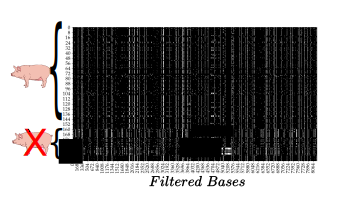
\includegraphics[width=0.85\textwidth]{Sequences.png}
\caption{SNP sequences of Salmonella enterica samples used in this work.
The x-axis shows the genome bases and the y-axis the corresponding sample (210 samples in total).
The black dots are related to a base without mutation (in relation to the genome reference), while the with dots are the mutation (SNPs) identified.
The first 159 rows contains the genome sequences related to pigs, i.e the sequences obtained by a pig which host the bacteria, and the following ones contains sequences of other animals.
Also with naked eyes we can see the differences between the two data types.
}
\label{fig:SNPsAle}
\end{figure}

First of all, we filtered our data removing from each genome a base if it was not mutated in each sample.
In this way we reduced the number of bases to $8189\,bp$.
A graphical representation of these samples is given in Fig.~\ref{fig:SNPsAle}.
The dataset was divided in training and test sets using a stratified cross-validation procedure to guarantee a proportional subdivision of the samples into the two classes.
The algorithm hyper-parameters were tuned on the training set in relation to the performances obtained using a internal stratified 10-fold cross-validation: in each fold the training was performed using a sequence of hyper-parameters and the performances evaluated on the corresponding test set; the hyper-parameters configuration which obtained the best performances on the full training set was chosen as best one.
We use our custom \emph{Score} library for the performance evaluation.
Considering the unbalanced sample quantities the Matthews Correlation Coefficient (MCC) was chosen as good score indicator for the evaluation.

\end{document}

\documentclass{standalone}

\begin{document}

\subsection[Results]{Results}\label{rfbp:snp_result}



\end{document}


\end{document}
